% Options for packages loaded elsewhere
\PassOptionsToPackage{unicode}{hyperref}
\PassOptionsToPackage{hyphens}{url}
%
\documentclass[
  12pt,
]{article}
\title{The Effect of Race, Income, and Vulnerability on FEMA Hazard
Mitigation Funding}
\usepackage{etoolbox}
\makeatletter
\providecommand{\subtitle}[1]{% add subtitle to \maketitle
  \apptocmd{\@title}{\par {\large #1 \par}}{}{}
}
\makeatother
\subtitle{\url{https://github.com/langstonalex/Alexander_ENV872_EDA_FinalProject.git}}
\author{Langston Alexander}
\date{}

\usepackage{amsmath,amssymb}
\usepackage{lmodern}
\usepackage{iftex}
\ifPDFTeX
  \usepackage[T1]{fontenc}
  \usepackage[utf8]{inputenc}
  \usepackage{textcomp} % provide euro and other symbols
\else % if luatex or xetex
  \usepackage{unicode-math}
  \defaultfontfeatures{Scale=MatchLowercase}
  \defaultfontfeatures[\rmfamily]{Ligatures=TeX,Scale=1}
  \setmainfont[]{Times New Roman}
\fi
% Use upquote if available, for straight quotes in verbatim environments
\IfFileExists{upquote.sty}{\usepackage{upquote}}{}
\IfFileExists{microtype.sty}{% use microtype if available
  \usepackage[]{microtype}
  \UseMicrotypeSet[protrusion]{basicmath} % disable protrusion for tt fonts
}{}
\makeatletter
\@ifundefined{KOMAClassName}{% if non-KOMA class
  \IfFileExists{parskip.sty}{%
    \usepackage{parskip}
  }{% else
    \setlength{\parindent}{0pt}
    \setlength{\parskip}{6pt plus 2pt minus 1pt}}
}{% if KOMA class
  \KOMAoptions{parskip=half}}
\makeatother
\usepackage{xcolor}
\IfFileExists{xurl.sty}{\usepackage{xurl}}{} % add URL line breaks if available
\IfFileExists{bookmark.sty}{\usepackage{bookmark}}{\usepackage{hyperref}}
\hypersetup{
  pdftitle={The Effect of Race, Income, and Vulnerability on FEMA Hazard Mitigation Funding},
  pdfauthor={Langston Alexander},
  hidelinks,
  pdfcreator={LaTeX via pandoc}}
\urlstyle{same} % disable monospaced font for URLs
\usepackage[margin=2.54cm]{geometry}
\usepackage{longtable,booktabs,array}
\usepackage{calc} % for calculating minipage widths
% Correct order of tables after \paragraph or \subparagraph
\usepackage{etoolbox}
\makeatletter
\patchcmd\longtable{\par}{\if@noskipsec\mbox{}\fi\par}{}{}
\makeatother
% Allow footnotes in longtable head/foot
\IfFileExists{footnotehyper.sty}{\usepackage{footnotehyper}}{\usepackage{footnote}}
\makesavenoteenv{longtable}
\usepackage{graphicx}
\makeatletter
\def\maxwidth{\ifdim\Gin@nat@width>\linewidth\linewidth\else\Gin@nat@width\fi}
\def\maxheight{\ifdim\Gin@nat@height>\textheight\textheight\else\Gin@nat@height\fi}
\makeatother
% Scale images if necessary, so that they will not overflow the page
% margins by default, and it is still possible to overwrite the defaults
% using explicit options in \includegraphics[width, height, ...]{}
\setkeys{Gin}{width=\maxwidth,height=\maxheight,keepaspectratio}
% Set default figure placement to htbp
\makeatletter
\def\fps@figure{htbp}
\makeatother
\setlength{\emergencystretch}{3em} % prevent overfull lines
\providecommand{\tightlist}{%
  \setlength{\itemsep}{0pt}\setlength{\parskip}{0pt}}
\setcounter{secnumdepth}{5}
\ifLuaTeX
  \usepackage{selnolig}  % disable illegal ligatures
\fi

\begin{document}
\maketitle

\newpage
\tableofcontents 
\newpage
\listoftables 
\newpage
\listoffigures 
\newpage

\hypertarget{rationale-and-research-questions}{%
\section{Rationale and Research
Questions}\label{rationale-and-research-questions}}

Climate change, primarily through thermal-expansion and melting polar
icecaps, could cause as much as 20 inches of sea-level rise. This amount
of sea-level rise will bring with it significant increases in flooding
throughout the coastal plain of North Carolina, impacting thousands of
peoples homes and businesses and causing millions of dollars in lost
economic potential. Although greenhouse gas mitigation will help to
avoid the worst possible outcomes of sea-level rise, as much as a 26\%
increase in flooding will occur due to historic emissions. Communities
must adapt to an increase in flood frequency if these baked in damages
are to be avoided.

Currently, the Federal Emergency Management Agency (FEMA) manages
federal policy on natural hazard mitigation and adaptation. Through a
variety of competitive grant programs, FEMA funds local efforts to
strengthen infrastructure, buildings, ecosystems, and services against
oncoming flooding. Recently, though, studies have shown that these grant
programs do not always end up in the hands of those most vulnerable. In
this paper, I will investigate whether FEMA hazard mitigation funding is
predicted by levels of race, income, or physical vulnerability for
counties in coastal North Carolina. The 20 coastal counties I
investigate in this paper are designated as coastal under North
Carolina's Coastal Area Management Act.

\hypertarget{question-1-is-amount-of-fema-hazard-mitigation-assistance-predicted-by-race-income-or-vulnerability-in-coastal-nc-counties}{%
\subsection{Question 1: Is amount of FEMA hazard mitigation assistance
predicted by race, income, or vulnerability in coastal NC
counties?}\label{question-1-is-amount-of-fema-hazard-mitigation-assistance-predicted-by-race-income-or-vulnerability-in-coastal-nc-counties}}

\newpage

\hypertarget{dataset-information}{%
\section{Dataset Information}\label{dataset-information}}

The data for this paper was sourced from FEMA and the U.S. Census. From
FEMA I used their Hazard Mitigation Assistance Projects dataset which
lists every hazard mitigation project funded through FEMA across the
U.S. from 1970-2022 by state and county, and listing the total dollars
spent on the project. I subsetted this data to only include the coastal
counties of North Carolina and summed the total amount spent on hazard
mitigation for each county. I then divided this total funding amount by
the total population of the county to get funding per capita. I did this
to try and counteract the bias toward more populated areas receiving
more funding.

From the U.S. Census I pulled racial, housing, and economic data by
county, again subsetting by coastal North Carolina counties. For the
racial component I used the decennial Census data on raw number of
Black, non-white Hispanic, Asian, other minorities by counties. I summed
these populations together, divided by the total population in a county
and multiplied by 100 to get the percentage of a county made up of
minorities.

For housing I simply used the raw number of mobile homes by county from
the U.S. Census. I used the number of mobile homes to operationalize the
concept of physical vulnerability. Mobile homes are some of the most
vulnerable to flooding and are often located in less desirable areas
that may be susceptible to flooding.

For economic data I used income per capita data by county from the U.S
Census.

Once cleaned and wrangled, I combined these datasets by county.

To get county spatial data, I used the North Carolina county spatial
dataset we used in class. I combined these datasets to create a single
dataset with all spatial, racial, economic, and housing data.

In Table 1 below see how these variables range across the 20 coastal
counties.

\begin{longtable}[]{@{}ll@{}}
\caption{Summary Statistics for NC Coastal Counties}\tabularnewline
\toprule
\endhead
Average\_Pop & 53198 \\
Max\_Pop & 225702 \\
Min\_Pop & 3245 \\
Average\_Minority\_Percent & 28 \\
Max\_Minority\_Pop\_Percent & 62 \\
Min\_Minority\_Pop\_Percent & 6.3 \\
Average\_Number\_Mobile\_Homes & 4366 \\
Max\_Number\_Mobile\_Homes & 19667 \\
Min\_Number\_Mobile\_Homes & 573 \\
Average\_Income\_PerCap & 27229 \\
Max\_Income\_PerCap & 34578 \\
Min\_Income\_PerCap & 18245 \\
Average\_HMA\_Funding & 8135424 \\
Max\_HMA\_Funding & 31032321 \\
Min\_HMA\_Funding & 10000 \\
\bottomrule
\end{longtable}

\newpage

\hypertarget{exploratory-analysis}{%
\section{Exploratory Analysis}\label{exploratory-analysis}}

I explored this data set through a series of bar charts and maps.

For each variable I created a bar chart by county to see how counties
compared to each other in terms of FEMA funding per capita (Figure 1),
minority populations (Figure 2), number of mobile homes(Figure 3), and
income per capita(Figure 4). From each of these bar charts we see a wide
range between the 20 counties. For example, in terms of FEMA funding per
capita Perquimans County has received \$10,000 while Beaufort County has
received over \$30 million. While differences in the counties are
evident with these bar charts, it is unclear if there is any connections
between the different variables.

To visually explore patterns between these four variables, I constructed
3 maps with FEMA funding per capita as the base layer and each of the 3
independent variables layered on top. Again, most of these maps do not
show any discernible pattern. In Figure 5, we see that counties with
both high and low percentages of minority populations receive less
funding than those with middling minority populations. In Figure 6, we
begin to see a pattern where counties with low numbers of mobile homes
receive more funding per capita. But, it is hard to make out how strong
this relationship is. In Figure 7, there is again a slight pattern where
poorer counties may be getting more funding per capita, but again the
pattern is hard to discern.

\begin{figure}
\centering
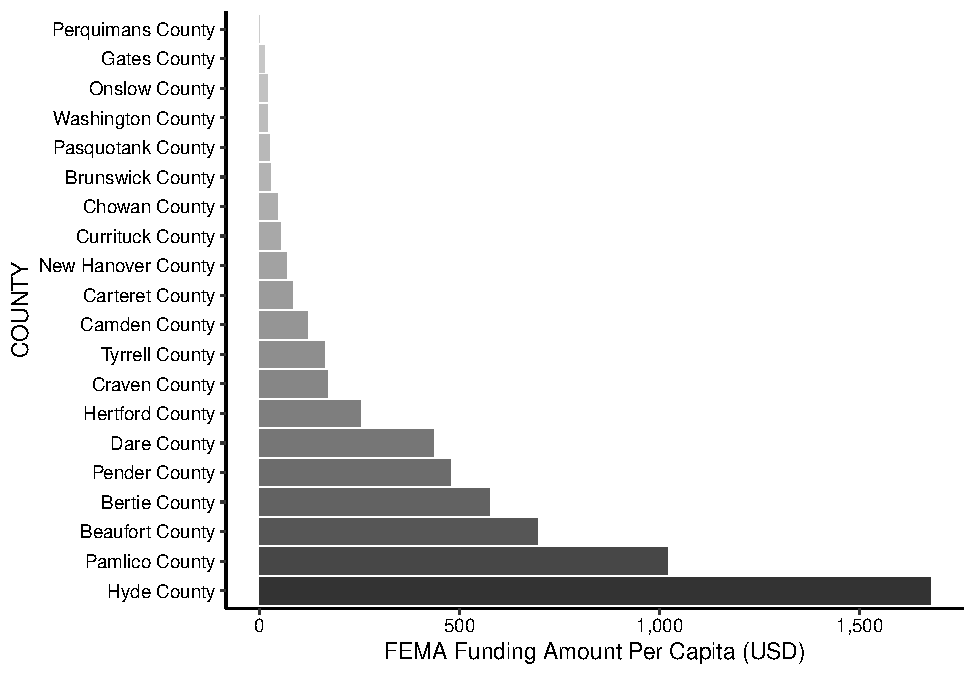
\includegraphics{Alexander_ENV872_Project_files/figure-latex/bar chart1-1.pdf}
\caption{FEMA Funding Per Capita for Hazard Mitigation By County}
\end{figure}

\begin{figure}
\centering
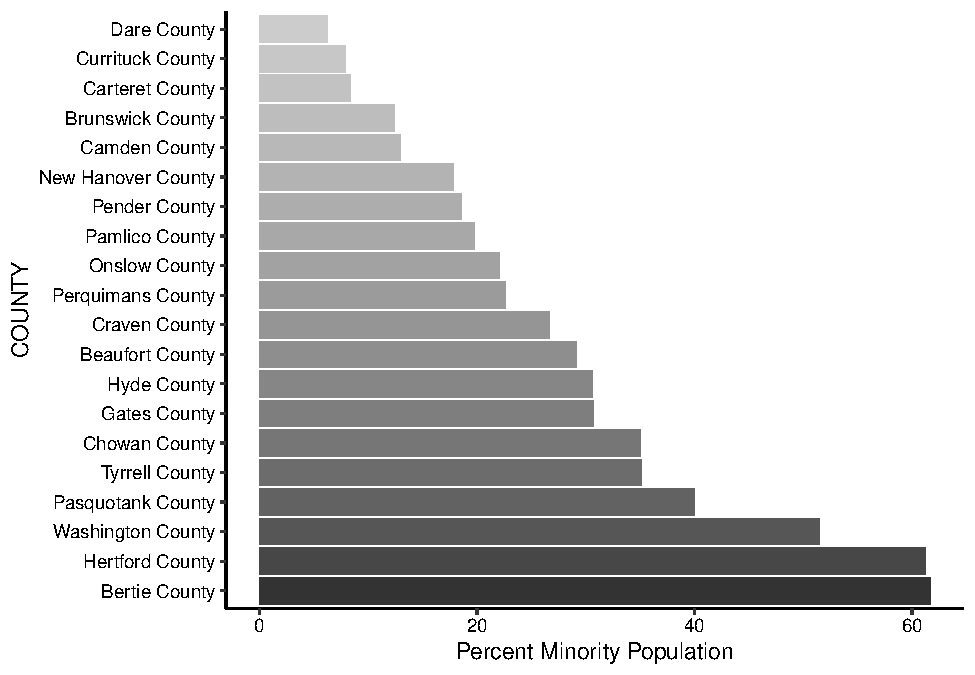
\includegraphics{Alexander_ENV872_Project_files/figure-latex/bar chart2-1.pdf}
\caption{Percent Minority By County}
\end{figure}

\begin{figure}
\centering
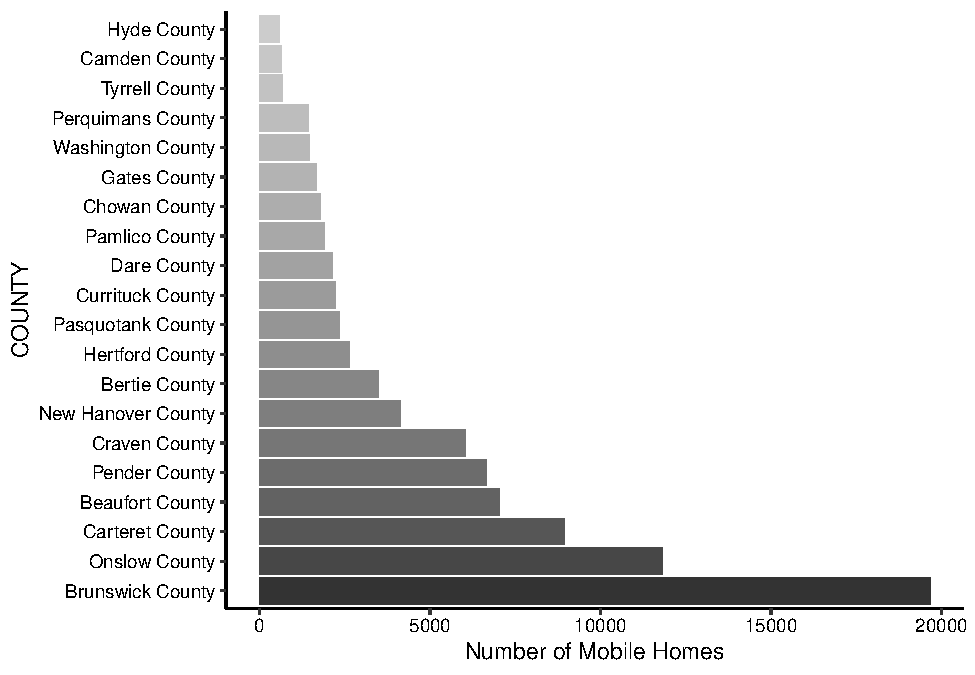
\includegraphics{Alexander_ENV872_Project_files/figure-latex/bar chart3-1.pdf}
\caption{Total Number of Mobile Homes By County}
\end{figure}

\begin{figure}
\centering
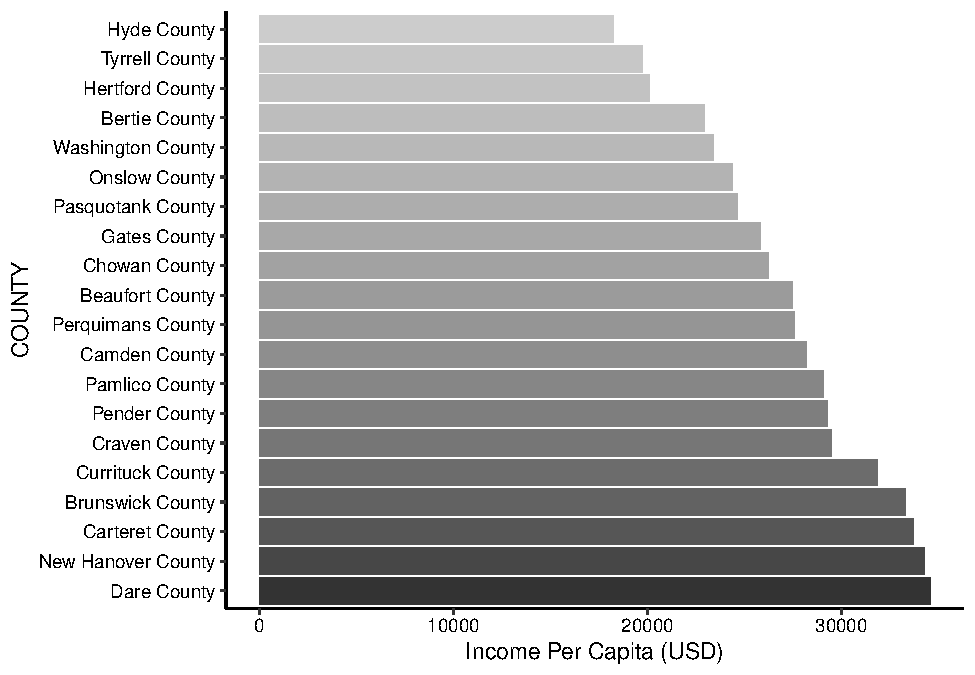
\includegraphics{Alexander_ENV872_Project_files/figure-latex/bar chart4-1.pdf}
\caption{Income Per Capita By County}
\end{figure}

\begin{figure}
\centering
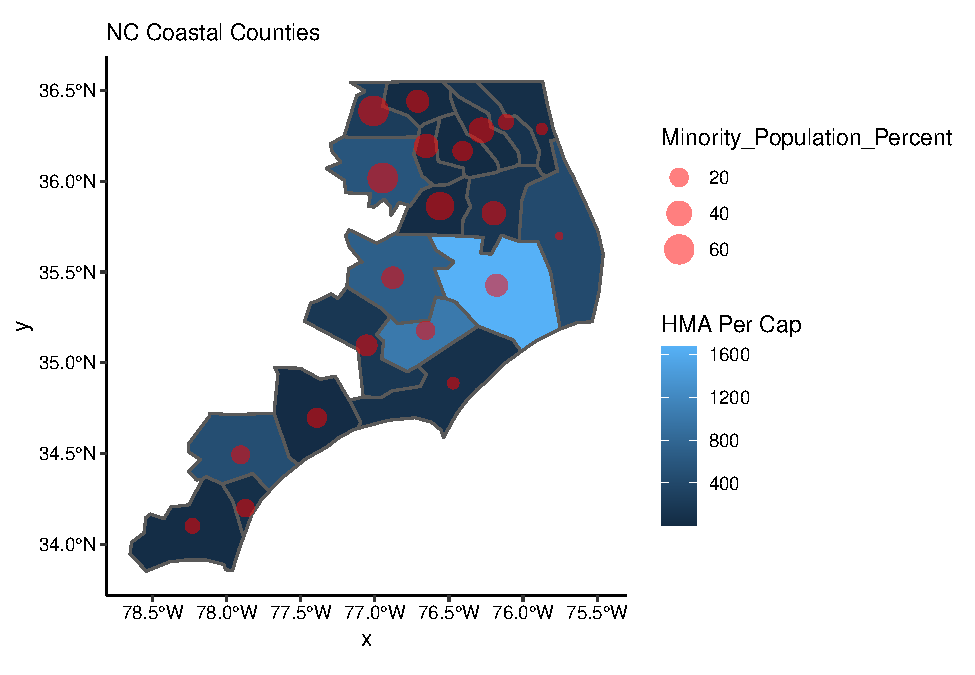
\includegraphics{Alexander_ENV872_Project_files/figure-latex/map1-1.pdf}
\caption{Hazard Mitigation Assistance and Minority Population Percent}
\end{figure}

\begin{figure}
\centering
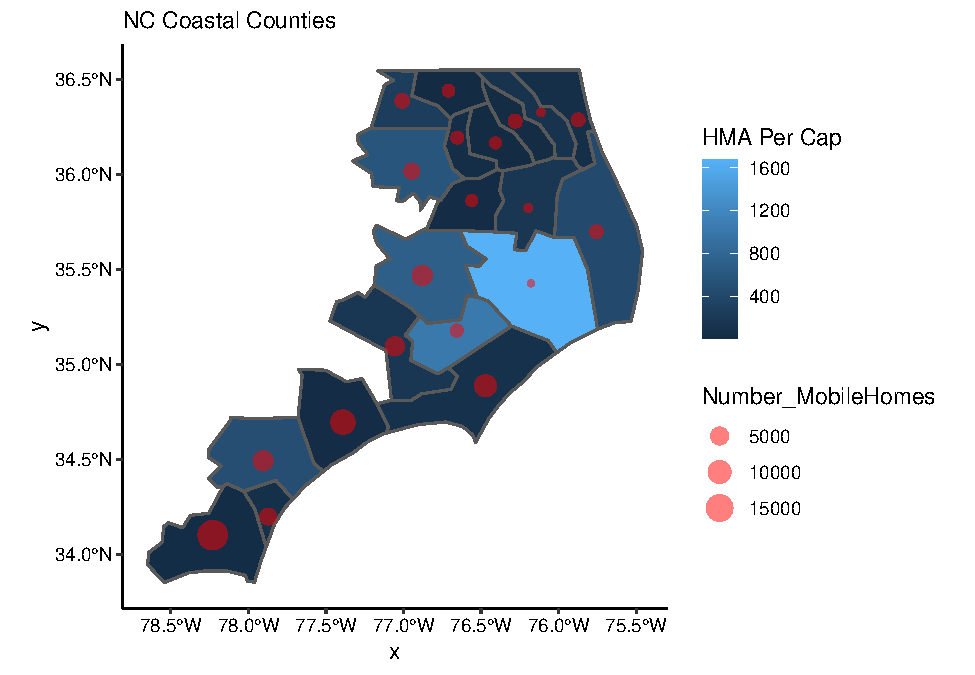
\includegraphics{Alexander_ENV872_Project_files/figure-latex/map2-1.pdf}
\caption{Hazard Mitigation Assistance Per Capita and Number of Mobile
Homes}
\end{figure}

\begin{figure}
\centering
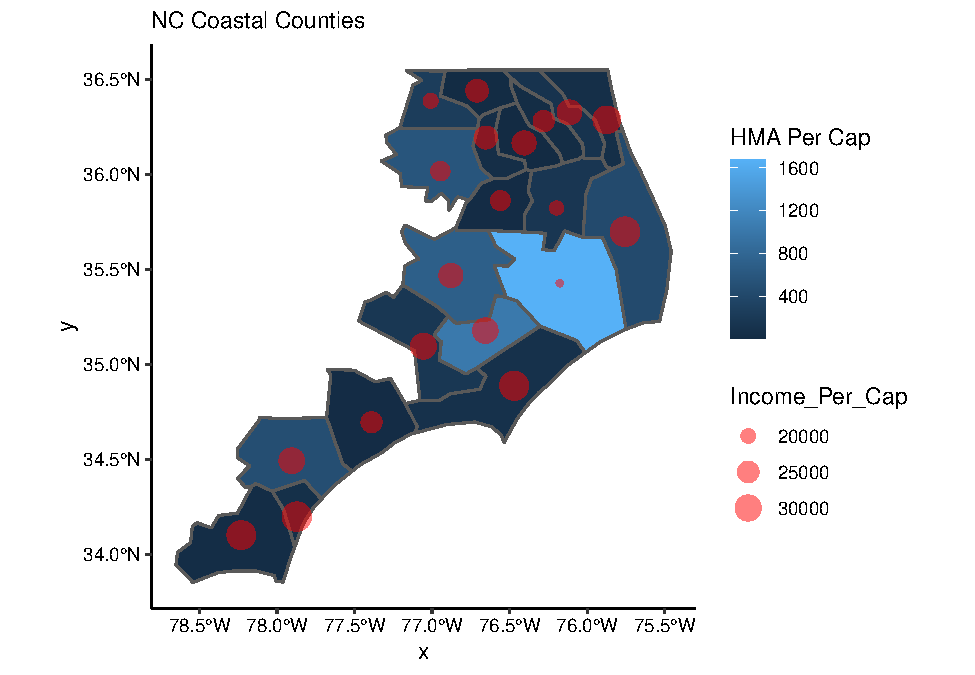
\includegraphics{Alexander_ENV872_Project_files/figure-latex/map3-1.pdf}
\caption{Hazard Mitigation Assistance and Income Per Capita}
\end{figure}

\newpage

\hypertarget{analysis}{%
\section{Analysis}\label{analysis}}

To further test the relationship between FEMA funding per capita and
percent minority, income per capita, and number of mobile homes I ran a
multi-linear regression. None of the 3 independent variables had
p-values less than 0.05 (minority population = 0.25, income per capita =
0.12, \# mobile homes = 0.69) meaning that for each we cannot reject the
null hypothesis that the independent variable suggesting there is no
statistical relationship. The R-Squared was 0.18 suggesting the
independent variables only explained 18\% of the variance in the
dependent variable.

To see if the data fit the model in the first place, I ran a residual
vs.~fitted plot, normal Q-Q plot, scale-location plot, and a residual
vs.~leverage plot.

\begin{figure}
\centering
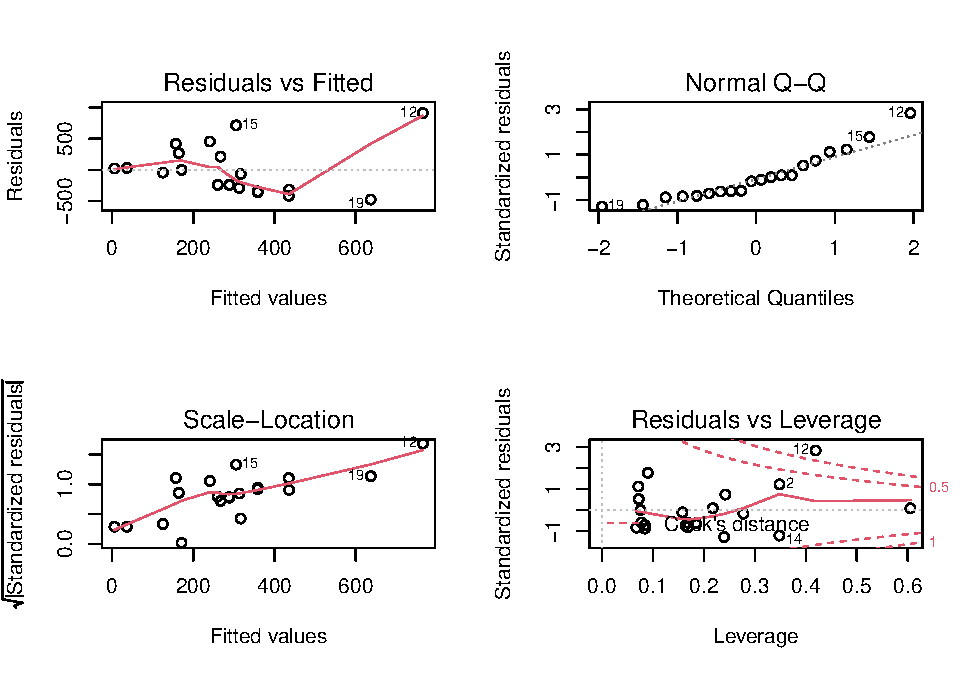
\includegraphics{Alexander_ENV872_Project_files/figure-latex/regression-1.pdf}
\caption{Fit of Model Graphs}
\end{figure}

\newpage

\hypertarget{summary-and-conclusions}{%
\section{Summary and Conclusions}\label{summary-and-conclusions}}

\end{document}
